\documentclass[12pt]{article}
\usepackage[a4paper, total={7.5in, 11in}]{geometry}
\usepackage{array}
\usepackage{graphicx, subfig, wrapfig, fancyhdr, lastpage, multicol ,color,arydshln,makecell}

\newcommand\headerMe[2]{\noindent{}#1\hfill#2}
\usepackage[mathscr]{euscript}
\usepackage{tabularray}

\setlength{\columnseprule}{1pt}
\def\columnseprulecolor{\color{blue}}


\pagestyle{fancy}
\fancyhf{}

\cfoot{ \vspace{-0.8cm}\em{Page \thepage \hspace{1pt} / \pageref{LastPage}}}
\begin{document}

\headerMe{Royaume du Maroc}{année scolaire \emph{2024-2025}}\\
\headerMe{Ministère de l'Éducation nationale, }{  Professeur :\emph{Zakaria Haouzan}}\\
\headerMe{du Préscolaire et des Sports}{Établissement : \emph{Lycée SKHOR qualifiant}}\\
%\vspace{-1cm}
\begin{center}
Devoir Surveillé  N°3 - S1 \\
    2ème année baccalauréat Sciences physiques\\
Durée 2h00
\\
    \vspace{.2cm}
\hrulefill
\Large{Chimie 7pts - 45min}
\hrulefill\\

    %\emph{Les deux parties sont indépendantes}
\end{center}
%end Headerss------------------------
%__________________Chimie ______________________-
%%%%%%%+_+_+_+_+_+_+_+_+_Partie1

 \section*{Partie 1 : Etude d’une solution aqueuse d’un acide carboxylique\dotfill(7pts)-45min }
%\begin{wrapfigure}{r}{0.16\textwidth}
	%\vspace{-1.2cm}
%%\begin{center}
  %%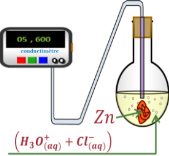
\includegraphics[width=0.16\textwidth]{./img/chimie01.png}
%%\end{center}
%\end{wrapfigure}



L'acide lactique est un acide organique qui joue un rôle important dans les divers processus biochimiques.
L'acide lactique de formule CH\textsubscript{3}CHOHCOOH, est produit par fermentation du lactose du lait à l'aide des bactéries. La teneur d'un lait en acide lactique est un indice de sa fraicheur. 

Un lait est considéré comme frais, si la concentration massique C\textsubscript{m} en acide lactique ne dépasse pas $1,8 g.L\textsuperscript{-1}$.

Le but de cet exercice est de déterminer l'acidité d'un lait après quelques jours de sa conservation dans une bouteille.

Pour simplifier, on notera le couple (CH\textsubscript{3}CHOHCOOH/CH\textsubscript{3}CHOHCOO\textsuperscript{-}) par (AH/A\textsuperscript{-}) et on considère que seul l'acide lactique est responsable de l'acidité.

On donne :
\begin{itemize}
    \item Masse molaire moléculaire de l'acide lactique : M(C\textsubscript{3}H\textsubscript{6}O\textsubscript{3}) = 90 g.mol\textsuperscript{-1}
    \item Produit ionique de l'eau à 25°C : K\textsubscript{e} = 10\textsuperscript{-14}
\end{itemize}

1- On verse dans un bécher, un volume V\textsubscript{A} = 20 mL d'une solution aqueuse (S\textsubscript{A}) d'acide lactique de concentration molaire C\textsubscript{A} = 2,0·10\textsuperscript{-2} mol.L\textsuperscript{-1}, puis on y ajoute un volume V\textsubscript{B} = 5,0 mL d'une solution aqueuse (S\textsubscript{B}) d'hydroxyde de sodium (Na\textsuperscript{+}\textsubscript{(aq)} + HO\textsuperscript{-}\textsubscript{(aq)}) de concentration molaire C\textsubscript{B} = 5,0·10\textsuperscript{-2} mol.L\textsuperscript{-1}.

La mesure du pH du mélange donne : pH = 4,0.

	\begin{tabular}{c | c}
		0,5 & \makecell[l]{\textbf{1.1. } Ecrire l'équation modélisant la réaction ayant lieu.}\\

		1,5 & \makecell[l]{\textbf{1.2. } Construire le tableau d'avancement de cette transformation, et déterminer la valeur de son \\taux d'avancement final $\tau$. Conclure ?}\\

      1,5 & \makecell[l]{\textbf{1.3. } Montrer que la constante pK\textsubscript{A} du couple (acide lactique/ion lactate) s'écrit :\\\hspace{2cm}
    $pK_A = pH + \log \left(\frac{C_A \cdot V_A}{C_B \cdot V_B} - 1\right)$
    Calculer la valeur de $pK_{A}$.}\\
						\end{tabular}


\textbf{2- Détermination de la concentration massique C\textsubscript{m} d'un lait :}

On verse dans un bécher, un volume V = 20 mL d'un lait (S), et on le neutralise à l'aide de la solution aqueuse précédente d'hydroxyde de sodium, en utilisant le dispositif du dosage. L'équivalence est atteinte lorsque le volume de la solution d'hydroxyde de sodium versé est V\textsubscript{BE} = 10 mL.

La solution S\textsubscript{a} est préparée par dissolution de l'acide AH dans l'eau. La mesure du pH de la solution S\textsubscript{a} donne : pH = 2,88.


	\begin{tabular}{c | c}
		0,75 & \makecell[l]{\textbf{2.1. } Tracez le schéma du dosage permettant de neutraliser l'acide lactique dans le lait à l'aide\\ d'une solution d'hydroxyde. Assurez-vous de préciser le nom de chaque matériel utilisé}\\

		1 & \makecell[l]{\textbf{2.2. } Calculer la concentration massique C\textsubscript{m} en acide lactique dans le lait (S). Conclure.}\\

						\end{tabular}


\textbf{3. Le pH du mélange à l'équivalence est : pH\textsubscript{E} = 8,0.}


	\begin{tabular}{c | c}
		0,5 & \makecell[l]{\textbf{3.1. } Indiquer, l'indicateur le plus convenable à ce dosage.}\\

    1,25 & \makecell[l]{\textbf{3.2. } Calculer le rapport $\frac{[A^-]}{[AH]}$ des concentrations, dans la solution obtenue à l'équivalence.\\ Déduire l'espèce prédominante.}\\

						\end{tabular}


\begin{center}
  \begin{tabular}{ |c| c|}
\hline
\textbf{Incicateur coloré} &\textbf{ Zone de virage}\\\hline
    Rouge de méthyle  & [4,2 - 6,2] \\\hline
    Rouge de phénol  & [6,6 - 8,4] \\\hline
    phénolphtaléine  & [8,2 - 10] \\\hline

\end{tabular}
\end{center}
%\hrulefill
%\Large{Physique 13pts/78min}
%\hrulefill\\
\newpage
\begin{center}
    %\vspace{.60cm}
\hrulefill
\Large{Physique 13pts - 75min}
\hrulefill\\
    \emph{Les  parties sont indépendantes}
\end{center}

%\vspace{-1cm}
\section*{Partie 1 : Vérification de la capacité d'un condensateur C \dotfill(6,25pts)}

\begin{wrapfigure}[9]{r}{0.25\textwidth}
  \begin{center}
	  \vspace{-1cm}
	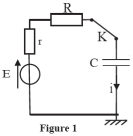
\includegraphics[width=0.19\textwidth]{./img/img01.png}
	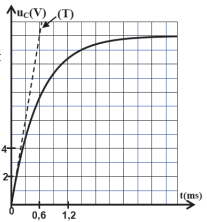
\includegraphics[width=0.25\textwidth]{./img/img02.png}
  \end{center}
\end{wrapfigure}
On réalise le circuit électrique schématisé
sur la figure 1 qui comporte :
\begin{itemize}
\item Un générateur de tension de f.e.m. (E). Deux conducteurs ohmiques de
résistance $r =20\Omega$ et R et Un condensateur de capacité C
initialement déchargé .
\end{itemize}
A un instant de date $t =0$, on place l’interrupteur K en
position (1). Un système d’acquisition informatisé permet de
tracer la courbe d’évolution de la tension $u_C(t)$. La droite (T)
représente la tangente à la courbe à la date $t=0$.

\begin{tabular}{c|l}
	1 & \makecell[l]{\textbf{1.1. }Etablir l’équation différentielle vérifiée par $u_C (t)$.}\\

	1 & \makecell[l]{\textbf{1.2. }Trouver les expressions de A et de $\tau$, pour que \\$u_C(t)=A.(1 -e^{-\frac{t}{\tau}})$ soit solution de cette équation différentielle.}\\
	
	1 & \makecell[l]{\textbf{1.3. }L’intensité du courant électrique s’écrit sous forme $i(t)=I_0.e^{-\frac{t}{\tau}}.$\\Trouver l’expression de $I_0$ en fonction de E, r et R. }\\
	
	1 & \makecell[l]{\textbf{1.4. }En exploitant la courbe,Trouver la valeur de la résistance R \\sachant que $I_0 = 0,20A$.  }\\
	
	1 & \makecell[l]{\textbf{1.5. }En exploitant la courbe,Déterminer la valeur de $\tau$.  }\\
	0,5 & \makecell[l]{\textbf{1.6. }Vérifier que la capacité du condensateur est $C=10\mu.F$. }\\
	0,75 & \makecell[l]{\textbf{1.7. }Trouver l’énergie E emmagasinée par le condensateur à \\l’instant $t = \frac{\tau}{2}$. }\\
	\end{tabular}

\section*{Partie 2 :Détermination expérimentale de la capacité d'un condensateur}


\begin{wrapfigure}[11]{r}{0.25\textwidth}
  \begin{center}
	  \vspace{-3cm}
	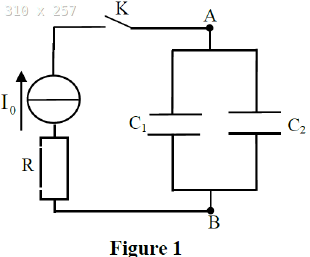
\includegraphics[width=0.25\textwidth]{./img/circuit00.png}
	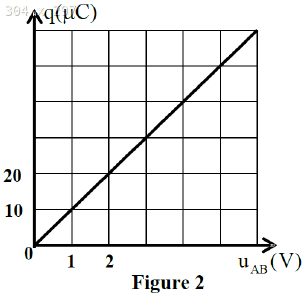
\includegraphics[width=0.25\textwidth]{./img/circuit01.png}
  \end{center}
\end{wrapfigure}

\textbf{1. En utilisant un générateur de courant}

Un premier groupe d'élèves d'une classe réalise, sous les directives du professeur, le montage expérimental de la figure 1 constitué des éléments suivants
\begin{itemize}
    \item un générateur idéal de courant qui alimente le circuit par un courant électrique d'intensité I\textsubscript{0}
    \item un conducteur ohmique de résistance R et deux condensateurs (c\textsubscript{1}) et (c\textsubscript{2}) montés en parallèle, respectivement de capacités $C_{1}=7,5\mu F$ et $C_{2}$ inconnue
\end{itemize}

À l'instant t\textsubscript{0}=0, un élève ferme le circuit. A l'aide d'un système d'acquisition informatisé, le groupe d'élèves obtient la courbe des variations de la charge q du condensateur équivalent à l'association des deux condensateurs (c\textsubscript{1}) et (c\textsubscript{2}) en fonction de la tension U\textsubscript{AB} (figure 2).



	\begin{tabular}{c | c}
		0,75 & \makecell[l]{\textbf{2.1. } Quel est l'intérêt de monter des condensateurs en parallèle ?}\\

		1 & \makecell[l]{\textbf{2.2. } En exploitant la courbe de la figure 2, déterminer la valeur de la capacité C\textsubscript{eq} du \\condensateur équivalent aux deux condensateurs (c\textsubscript{1}) et (c\textsubscript{2}).}\\
 1 & \makecell[l]{\textbf{2.3 } En déduire la valeur de la capacité C\textsubscript{2}. Etablir l'équation différentielle vérifiée par l'intensité \\du courant électrique i(t) traversant le circuit.}
						\end{tabular}

\newpage
            
\subsection*{Partie 3: En étudiant la réponse du dipôle RC à un échelon de tension}

Un deuxième groupe d'élèves de la même classe réalise le montage représenté par la figure 3 constitué par:
\begin{itemize}
    \item Un générateur idéal de tension de force électromotrice E
    \item Un conducteur ohmique de résistance $R = 1600\Omega$
    \item Le condensateur précédent de capacité C\textsubscript{2}
    \item Un interrupteur K à double position
\end{itemize}

  \begin{center}
	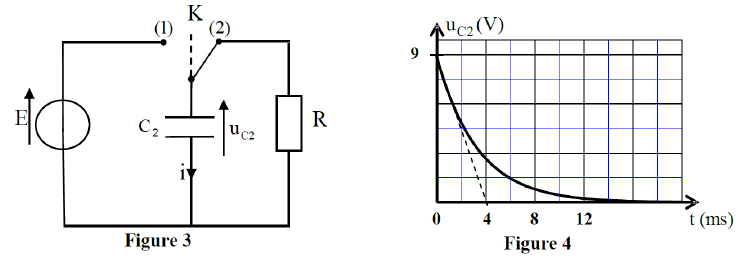
\includegraphics[width=0.75\textwidth]{./img/circuit003.png}
  \end{center}
Après avoir chargé totalement le condensateur, un élève bascule l'interrupteur K sur la position (2) à l'instant t\textsubscript{0}=0. A l'aide d'un système d'acquisition informatisé, le groupe d'élèves obtient la courbe des variations de la tension U\textsubscript{C\textsubscript{2}}(t) aux bornes du condensateur (figure 4).

	\begin{tabular}{c | c}
		0,75 & \makecell[l]{\textbf{3.1. } Établir l'équation différentielle vérifiée par la tension U\textsubscript{C\textsubscript{2}}(t) au cours de la décharge \\du condensateur.}\\

		1 & \makecell[l]{\textbf{3.2. } La solution de cette équation différentielle est de la forme :
    \\$U_{C_2}(t) = \frac{E}{R} \cdot e^{-\frac{t}{\tau}}$
    \\Trouver l'expression de la constante de temps $\tau$ en fonction de R et \(C\textsubscript{2}\).}\\
 0,5 & \makecell[l]{\textbf{3.3 } Déterminer de nouveau la valeur de la capacité C\textsubscript{2}.}\\
 0,75 & \makecell[l]{\textbf{3.4 } Déterminer l'expression de la charge q(t) et l'expression de
l'intensité du courant i(t)}\\

 1 & \makecell[l]{\textbf{3.5 } Comment choisir la valeur de la résistance R pour avoir une décharge rapide}\\
						\end{tabular}
\end{document}
